\subsection{Charges}
\begin{itemize}
    \item The charges are $α_{\text{W}}, α_{\text{W}}, α_{\text{S}}$, for the weak, electromagnetic, and strong force, respectively.
    \item The product of the charges show how likely an interaction is to happen.
\end{itemize}

\subsubsection{Examples}
At the vertices in \cref{eq: charge_1}, we place the charge, $α_{\text{EM}}$, being proportional to the electromagnetic charge squared. 
\begin{equation}\label{eq: charge_1}
e^{-} γ \stackrel{α_{\text{EM}}}{→} e^{-} γ
\end{equation}

We do the same for the strong force in \cref{eq: charge_2}.
\begin{equation}\label{eq: charge_2}
  g \stackrel{α_{\text{S}}}{→} gg
\end{equation}

\subsection{Allowed Vertices (\cref{fig: feynman_diagram_vertices})}
\begin{itemize}
    \item A vertices is where the particle lines meet. 
    \item Processes can in theory be written in reverse. 
    \item Not all vertices are allowed. The $Q$-value must be negative, meaning the process must be energetically allowed.
    \item Quantities like charge, baryon number, lepton number,energy and strangeness must be conserved. 
    \item $e^{+} → e^{+}γ$ would not be allowed as we can pick a frame of reference where the electron is at rest, and the photon would have energy less than or equal to 0.
\end{itemize}

\begin{figure}[h!]
\centering
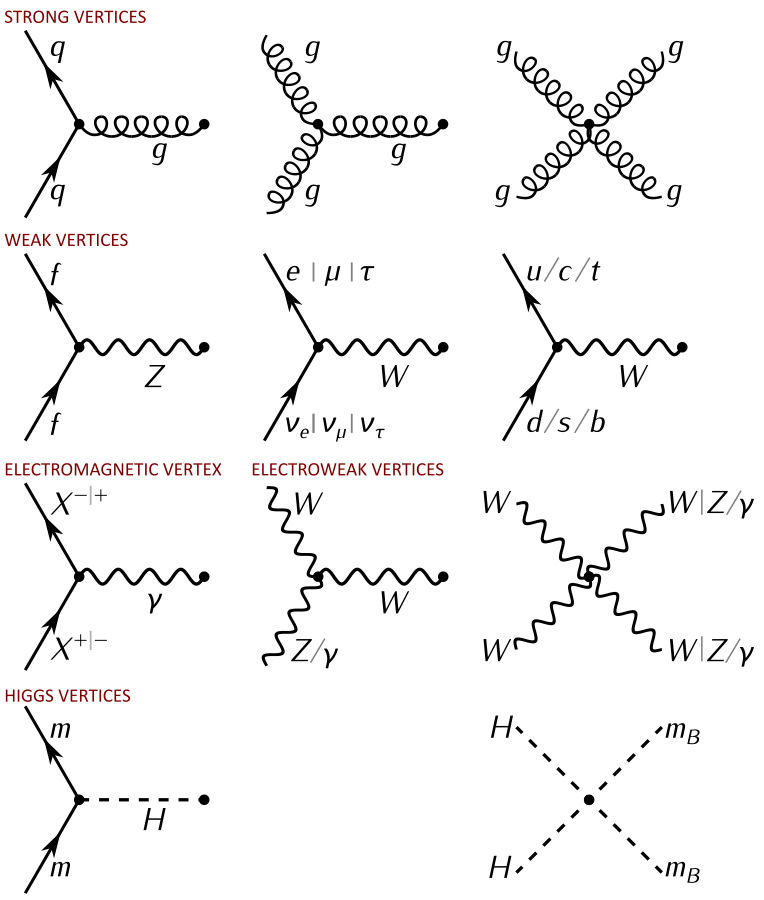
\includegraphics[width = \textwidth]{feynman_diagram_vertices.png}
\caption{Figure of allowed vertices in the Standard Model.}
\label{fig: feynman_diagram_vertices}
\end{figure}


We can change the time ordering in \cref{eq: charge_1}, to the following in \cref{eq: charge_3}. Here the photons comes in and interacts with the electron. This is a non-physical process, as the mass/energy of the system in a rest frame is not conserved. 
\begin{equation}\label{eq: charge_3}
  γ e^{-} \stackrel{α_{\text{EM}}}{→} e^{-} γ
\end{equation}

\subsubsection{Allowed EM Vertices}
\cref{eq: a_EM_v_1} is allowed as a part of a larger process, but not on its own. This is because the mass of the tauon can't increase or decrease, meaning the photon must have a mass (energy) of 0.
\begin{equation}\label{eq: a_EM_v_1}
τ^{+} → τ^{+}γ
\end{equation}

\cref{eq: a_EM_v_2} is allowed as a part of a larger process, but not on its own. Same as \cref{eq: a_EM_v_1}, where the mass of the anti charm quark can't increase or decrease, meaning the photon must have a mass (energy) of 0. 
\begin{equation}\label{eq: a_EM_v_2}
y \bar{c} → \bar{c}
\end{equation}

\cref{eq: a_EM_v_3} is allowed as a part of a larger process, but not on its own. A real photon does not have mass, meaning it cannot create a top quark and an anti-top quark. We could flip one of the vertices to be $γ \bar{t} → \bar{t}$ and we see this to be impossible. 
\begin{equation}\label{eq: a_EM_v_3}
γ → t\bar{t}
\end{equation}

\subsubsection{Allowed Strong Vertices}
\cref{eq: a_strong_v_1} Could be a part of a larger diagram, but can't represent a physical process on its own due to conservation of energy. 
\begin{equation}\label{eq: a_strong_v_1}
  g \bar{c} → \bar{c}
\end{equation}

\cref{eq: a_strong_v_2} This is a possible process, as the gluon can have a high enough mass for this to be possible. 
\begin{equation}\label{eq: a_strong_v_2}
  g → t \bar{t}
\end{equation}

\cref{eq: a_strong_v_3} This is a possible process, as the gluon can interact with it self
\begin{equation}\label{eq: a_strong_v_3}
  g → g g
\end{equation}


\subsubsection{Neutral Weak Vertices}
All vertices with the photon can be interchanged with the $Z^{0}$-boson but NOT the other way around. See \cref{eq: a_weak_v_1} for an example.
\begin{equation}\label{eq: a_weak_v_1}
  γ / Z^{0} → e^{+} e^{-}  
\end{equation}

The neutrino is electrically neutral, and does not interact with the photon, meaning the process in \cref{eq: a_weak_v_2} only works with a $Z^{0}$-boson.
\begin{equation}\label{eq: a_weak_v_2}
  ν_{μ} → ν_{μ}Z^{0}
\end{equation}

As the process is electrically neutral, the $Z^{0}$-boson can be created from the annihilation of a down-type quark and an anti-down-type quark, as seen in \cref{eq: a_weak_v_3}.
\begin{equation}\label{eq: a_weak_v_3}
  d \bar{d} → Z^{+}  
\end{equation}

\subsubsection{Charged Weak Vertices}
The $W^{±}$-boson can interact with all fermions, but as it has a charge, it changes the charge of the particles it interacts with. Net charge must be conserved, meaning the process in \cref{eq: a_weak_v_4} is allowed.
\begin{equation}\label{eq: a_weak_v_4}
  W^{-} → \bar{u} d
\end{equation}

To get zero charge, but keep the number of anti-fermions we can have the process in \cref{eq: a_weak_v_5}.
\begin{equation}\label{eq: a_weak_v_5}
  e^{+}W^{-} → \bar{ν}_{e}
\end{equation}

The electric charge of the $W^{±}$-boson can interact with the photon. This is seen in \cref{eq: a_weak_v_6}.
\begin{equation}\label{eq: a_weak_v_6}
  W^{+} → W^{+}γ
\end{equation}

Net charge is conserved, which allows the process in \cref{eq: a_weak_v_7}.
\begin{equation}\label{eq: a_weak_v_7}
  Z^{0} → W^{+}W^{-}  
\end{equation}

\subsubsection{Higgs Boson Vertices}
The Higgs boson interacts with the mass of fermions, but maybe not the mass of neutrinos. 

\cref{eq: a_higgs_v_1} is a possible process, as the Higgs boson can interact with the mass of the top quark.
\begin{equation}\label{eq: a_higgs_v_1}
  t \bar{t} → H
\end{equation}

\cref{eq: a_higgs_v_2} is a possible process, as the Higgs boson can create the muons, as charge is conserved. 
\begin{equation}\label{eq: a_higgs_v_2}
  H → μ^{+} μ^{-}
\end{equation}

\cref{eq: a_higgs_v_3} is possible, and dependant on the mass of the $Z^{0}$-boson.
\begin{equation}\label{eq: a_higgs_v_3}
Z_0 → Z^{0}H  
\end{equation}

The Higgs boson can interact with itself, as seen in \cref{eq: a_higgs_v_4}.
\begin{equation}\label{eq: a_higgs_v_4}
H → H H
\end{equation} 



